\def\auth{Carlos Salinas}
\def\tight{MA571: Qual Preparation}
\def\short{MA71 Qual Prep}
\def\class{MA571}
\def\subject{point-set topology}
\def\email{salinac@purdue.edu}

\documentclass[10pt,twoside]{article}

%% Base customization and variables
\usepackage[eucal]{clos-vars}

%% Formatting

%% Footnote style
\renewcommand*{\thefootnote}{\fnsymbol{footnote}}

%% Hyperref setup
\hypersetup{%
  breaklinks,%
  colorlinks=true,%
  linkcolor=black,%
  citecolor=black,%
  filecolor=black,%
  menucolor=black,%
  runcolor=black,%
  urlcolor=black,%
  pdftitle={\short},%
  pdfauthor={\auth},%
  pdfkeywords={\subject},%
  pdfsubject={\class},%
  pageanchor={false}%
}

%% Graphics path as it says
\graphicspath{{figures/}}

\begin{document}
\thispagestyle{empty}
\author{\href{mailto:\email}{\auth}}
\title{\tight}
\date{\today}

\maketitle
\tableofcontents

%% McClure Homework
\section{MA 571 Fall 2015}
% \thispagestyle{empty}
This is material from the course MA 571 as it was taught in the fall of
2015.%
\bigskip
\subsection{Homework}
Most of the homework is from \cite{munkres} with a few exercises
(especially those involving the quotient topology and manifolds) written by
McClure. Unless otherwise stated, whenever we quote a result, e.g.,
Theorems 1.1, it is understood to come from Munkre's \emph{Topology}.

Throughout these notes

\begin{tabular}{cl}
  \(\bbR\) & is the set of real numbers\\
  \(\bbC\) & is the set of complex numbers\\
  \(\bbQ\) & is the set of rational numbers\\
  \(\bbZ\) & is the set of the integers\\
  \(\bbZ^+\) & is the set of positive integers, that is, \(x\in\bbZ\) with
               \(x\geq 0\)\\
  \(\bbN\) & is the set of the natural numbers \(1,2,\dotsc\)\\
  \(A\setminus B\) & is the set difference of \(A\) and \(B\), that is, the
                     complement of \(A\cap B\) in \(A\)\\
  \(X\approx Y\)& means \(X\) and \(Y\) are homeomorphic\\
  \(f\simeq g\)& means \(f\) is homotopic to \(g\)\\
  \(X\simeq Y\)&means \(X\) and \(Y\) are homotopy equivalent\\
  \(G\cong H\)& means \(G\) and \(H\) are isomorphic as groups
\end{tabular}

\newpage
\subsubsection{Homework 1}
\setcounter{exercise}{0}
\setcounter{equation}{0}


%%% Local Variables:
%%% mode: latex
%%% TeX-master: "../MA571-Quals"
%%% End:

\subsection{Homework 2}

%%% Local Variables:
%%% mode: latex
%%% TeX-master: "../MA571-Quals"
%%% End:

\subsubsection{Homework 3}

%%% Local Variables:
%%% mode: latex
%%% TeX-master: "../MA571-Quals"
%%% End:

\subsubsection{Homework 4}

%%% Local Variables:
%%% mode: latex
%%% TeX-master: "../MA571-Quals"
%%% End:

\subsubsection{Homework 5}
\setcounter{exercise}{0}


%%% Local Variables:
%%% mode: latex
%%% TeX-master: "../MA571-Quals"
%%% End:

\subsection{Homework 6}

%%% Local Variables:
%%% mode: latex
%%% TeX-master: "../MA571-Quals"
%%% End:

\subsection{Homework 7}

%%% Local Variables:
%%% mode: latex
%%% TeX-master: "../MA571-Quals"
%%% End:

\subsubsection{Homework 8}
\setcounter{exercise}{0}


%%% Local Variables:
%%% mode: latex
%%% TeX-master: "../MA571-Quals"
%%% End:

\subsubsection{Homework 9}
\setcounter{exercise}{0}


%%% Local Variables:
%%% mode: latex
%%% TeX-master: "../MA571-Quals"
%%% End:

\subsection{Homework 10}

%%% Local Variables:
%%% mode: latex
%%% TeX-master: "../MA571-Quals"
%%% End:

\subsubsection{Homework 11}
\setcounter{exercise}{0}


%%% Local Variables:
%%% mode: latex
%%% TeX-master: "../MA571-Quals"
%%% End:

\subsubsection{Homework 12}

%%% Local Variables:
%%% mode: latex
%%% TeX-master: "../MA571-Quals"
%%% End:

\subsubsection{Homework 13}
\setcounter{exercise}{0}


%%% Local Variables:
%%% mode: latex
%%% TeX-master: "../MA571-Quals"
%%% End:


%% McClure Quals
\section{McClure}
\subsection{McClure: Summer 2006}
\setcounter{exercise}{0}
\setcounter{equation}{0}

\begin{problem}
  Let \(X\) be a connected space and let \(f\colon X\to Y\) be a function
  which is continuous and onto. Prove that \(Y\) is connected. (This is a
  theorem in Munkres---prove it from the definitions).
\end{problem}
\begin{solution}
  We will show that the only separation of \(Y\) is the trivial one.

  Let \(C,D\) be a separation of \(Y\). Then, \(C\) and \(D\) are open and
  \(Y=C\cup D\). Since \(f\) is continuous \(f^{-1}(C)\) and \(f^{-1}(D)\)
  are open in \(X\) and
  \[
    X=f^{-1}(Y)=f^{-1}(C\cup D)=f^{-1}(C)\cup f^{-1}(D).
  \]
  Since \(X\) is connected we have \(f^{-1}(C)=\emptyset,f^{-1}(D)=X\) or
  \(f^{-1}(C)=X,f^{-1}(D)=\emptyset\); we may, without loss of generality,
  assume that \(f^{-1}(C)=\emptyset\) and \(f^{-1}(D)=X\). But since \(f\)
  is onto, from elementary set theory, we have \(f(f^{-1}(C))=C\) and
  \(f(f^{-1}(D))=D\). Thus, it must be the case that \(C=\emptyset\) and
  \(D=Y\). It follows that the only separation of \(Y\) is the trivial
  separation and so \(Y\) is connected.
\end{solution}

\begin{problem}
  Let \(X\) be the Cartesian product \(\prod_{i=1}^\infty\bbR\) with the
  \emph{box topology} (recall that a basis for this topology consists of
  all sets of the form \(\prod_{i=1}^\infty U_i\), where \(U_i\) is open in
  \(\bbR\). Let \(f\colon\bbR\to X\) be the function which takes \(t\) to
  \((t,t,\ldots)\). Prove that \(f\) is not continuous.
\end{problem}
\begin{solution}
  We show that for some neighborhood \(U\) of \(\mathbf{0}\), \(f^{-1}(U)\)
  is not open in \(\bbR\) with the standard topology. Consider the set
  \[
    U=\prod_{n=1}^\infty U_n
  \]
  where \(U_n=(-1/n,1/n)\). Since each \(U_n\) is open in \(\bbR\), \(U\)
  is open in the box topology. Moreover, \(\mathbf{0}\in U\) since
  \(0\in U_n\) for all \(n\). Therefore, \(U\) is a neighborhood of
  \(\mathbf{0}\). Now, consider the preimage of \(U\) under \(f\),
  \(f^{-1}(U)\). We claim that \(f^{-1}(U)=\{0\}\). We have already seen
  that \(0\in f^{-1}(U)\) so \(\{0\}\subseteq f^{-1}(U)\). It remains to
  show that \(0\) is the only element in \(f^{-1}(U)\). Let
  \(x\in f^{-1}(U)\). We may, without loss of generality, assume that
  \(x>0\). Then, by the Archimedean property of \(\bbR\), there exist an
  natural number \(N\) such that \(1/N<x\). Then, for every \(n\geq N\),
  \(x\notin U_n\). This is a contradiction. Therefore \(x\leq 0\). A
  similar argument shows that \(x\geq 0\). Thus, \(x=0\). Since the
  preimage of \(f^{-1}(U)=\{0\}\) is not open in \(\bbR\), it follows that
  \(f\) is not continuous.
\end{solution}

\begin{problem}
  Let \(Y\) be a topological space. Let \(X\) be a set and let
  \(f\colon X\to Y\) be a function. Give \(X\) the topology in which the
  open sets are the empty set and the sets \(f^{-1}(V)\) with \(V\) open in
  \(Y\) (you do not have to verify that this is a topology). Let \(a\in X\)
  and let \(B\) be a closed set in \(X\) not containing \(a\). Prove that
  \(f(a)\) is not in the closure of \(f(B)\).
\end{problem}
\begin{solution}
  Seeking a contradiction, suppose that \(f(a)\in\overline{f(B)}\). Then,
  for every neighborhood \(V\) of \(f(a)\), \(V\cap f(B)\) is nonempty. Let
  \(y\in V\cap f(B)\). Then, there exist \(x\in B\) such that
  \(f(x)=y\). Moreover, \(f^{-1}(V)\) is, by definition, open in \(X\) and
  is a neighborhood of \(a\) with \(x\in f^{-1}(V)\cap B\). Since every
  neighborhood of \(a\) the preimage of some open subset of \(Y\), it
  follows that \(a\in B\). This is a contradiction. Therefore, it must be
  the case that \(f(a)\notin\overline{f(B)}\).
\end{solution}

For the next two problems, let \(P\) be the Cartesian product
\(\prod_{i=1}^\infty\{0,1\}\) with the usual Cartesian product
topology. (Note that \(\{0,1\}\) is a set with two points, it is not an
interval.)
\begin{problem}
  Prove that every function from the Cantor set \(C\) to \(P\) which is
  one-to-one, onto and continuous is a homeomorphism.
\end{problem}
\begin{solution}
  First, note that \(P\) is Hausdorff since \(\{0,1\}\) is a subspace of
  \(\bbR\) which is Hausdorff and the product of Hausdorff spaces equipped
  with the product topology is again Hausdorff.

  Moreover, since \(C=\bigcap_{n=1}^\infty A_n\) and each \(A_n\) is the
  disjoint union of a finite collection of closed intervals in \([0,1]\),
  \(C\) is closed since the intersection of a collection of closed sets is
  again closed. Then \(C\) is compact since it is a closed subspace of
  \([0,1]\), the latter a compact subspace of \(\bbR\).

  It follows from a theorem in chapter 23 that if \(f\colon C\to P\) is
  one-to-one, onto and continuous it is a homeomorphism since \(C\) is
  compact and \(P\) is Hausdorff.
\end{solution}

\begin{problem}
  \hfill
  \begin{enumerate}[label=(\alph*),noitemsep]
  \item Give a clear and specific description of a function from the Cantor
    set to \(P\) which is one-to-one and onto. You do not have to prove
    that your function is one-to-one and onto.
  \item Prove that the function you described in part (a) is
    continuous. (If it isn't continuous, go back and choose a different
    function that is).
  \end{enumerate}
\end{problem}
\begin{solution}
  For part (a) we take the following claim will be taken for granted: The
  set \(C\) consists of all term series of the form
  \[
    \sum_{n=1}^\infty\frac{a_n}{3^n}
  \]
  where \(a_n\in\{0,2\}\). Define a map \(f\colon C\to P\) by
  \[
    f\left(\sum_{n=1}^\infty\frac{a_n}{3^n}\right)=(a_1/2,a_2/2,\ldots).
  \]

  For part (b), to see that \(f\) is continuous note that
  \(\pi_n\circ f=a_n/2\) is multiplication on \(\bbR\) which is continuous
  on \(\bbR\), hence it is continuous on the subspace \(\{0,1\}\) of
  \(\bbR\). By the universal mapping property of the product topology (see
  the diagram below)
  \[
    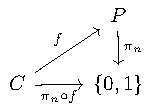
\includegraphics{aug06/aug06-prob5}
  \]
  since every projection of \(f\), \(\pi_n\circ f\) is continuous, it
  follows that \(f\) is continuous.
\end{solution}

\begin{problem}
  Let \(X\) and \(Y\) be topological spaces, let \(x_0\in X\), \(y_0\in Y\)
  and let \(f\colon X\to Y\) be a continuous function which takes \(x_0\)
  to \(y_0\).

  Is the following statement true? If \(f\) is one-to-one then
  \(f_*\colon\pi(X,x_0)\to \pi_1(Y,y_0)\) is one-to-one. Prove or give a
  counterexample (and if you give a counterexample, justify it). You may
  use anything in Munkres's book.
\end{problem}
\begin{solution}
  We provide a counter example. Let \(B^2\) be the open ball of radius
  \(1\) cenntered at \((0,0)\), \(S^1\) the circle of radius \(1\) centered
  at \((0,0)\) and fix \(x_0=(0,1)\) on \(S^2\) Then, the canonical
  inclusion \(\iota\colon S^1\to B^2\) is injective. However,
  \(\pi_1(S^1,x_0)\cong\bbZ\) whereas \(\pi_1(B^2,x_0)\cong \{0\}\) and no
  map \(f\colon\bbZ\to\{0\}\) is injective.
\end{solution}

\begin{problem}
  Let \(S^2\) be the \(2\)-sphere, that is, the following subspace of
  \(\bbR^3\): the set
  \[
    \left\{\,(x,y,z)\in\bbR^3:x^2+y^2+z^2=1\,\right\}.
  \]
  Let \(x_0\) be the point \((0,0,1)\) of \(S^2\).


  Use the Seifert--van Kampen theorem to prove that \(\pi_1(S^2,x_0)\) is
  the trivial group. You may use either of the two versions of the
  Seifert--van Kampen theorem given in Munkres's book. You will not get
  credit for any other method.
\end{problem}

\begin{solution}
  Let \(N\) and \(S\) denote the points \((0,0,1)\) and \((0,0,-1)\),
  respectively. Then the sets
  \[
    U=S^2\setminus\{N\}\qquad\text{and}\qquad V=S^2\setminus\{S\}
  \]
  are open in \(S^2\) and both contain the point \(x_0\). Now since
  \(U,V\approx\bbR\) via the stereographic projections
  \(\pi_N\colon N\to\bbR^2\), \(\pi_S\colon S\to\bbR^2\) we have
  \[
    \pi_1(U,x_0)\cong\pi_1(V,x_0)\cong\pi_1(\bbR^2,\pi_N(x_0))\cong\{0\}.
  \]
  Thus, by the Seifert--van Kampen theorem,
  \[
    \pi_1(S^2,x_0)\cong\frac{\pi_1(U,x_0)*\pi_1(V,x_0)}{N'}\cong\{0\}
  \]
  since \(\{0\}*\{0\}\cong\{0\}\) and any quotient of the trivial subgroup
  is trivial.
\end{solution}

%%% Local Variables:
%%% mode: latex
%%% TeX-master: "../MA571-Quals"
%%% End:

\include{mcclure/571-aug-07}
\subsection{McClure: Winter 2011}
\setcounter{exercise}{0}

\begin{problem}
  Let \(A\) be a subset of a topological space \(X\) and let \(B\) be a
  subset of \(A\). Prove that
  \(\bar A\setminus\bar B\subseteq\overline{A\setminus B}\).
\end{problem}
\begin{solution}
  Let \(x\in\bar A\setminus\bar B\), then \(x\) is in the closure of \(A\),
  but not in the closure of \(B\), i.e., there exists a neighborhood \(U\)
  of \(x\) such that \(U\cap B=\emptyset\) and \(U\cap A\neq\emptyset\). In
  particular, the latter shows that \(A\setminus B\neq\emptyset\) and so
  \(U\cap A\setminus B\neq\emptyset\). This is true for every neighborhood
  of \(x\in\bar A\setminus\bar B\). Thus, \(x\in\overline{A\setminus B}\).
\end{solution}

\begin{problem}
  Let \(G\) be a topological group (that is, a group with a topology for
  which the group operations are continuous) and let \(H\) be a subgroup of
  \(G\). Suppose that \(G\) is connected, that \(H\) is a normal subgroup
  of \(G\), and that the subspace topology on \(H\) is discrete. Prove that
  \(gh=hg\) for every \(g\in G\), \(h\in G\).
\end{problem}
\begin{solution}
  Fix \(h\in H\) and consider the map \(f_h \colon H\to H\) given by
  \(f_h(g)=ghg^{-1}\). Since \(H\) is normal in \(G\), \(ghg^{-1}\in H\)
  and since multiplication is continuous in \(G\) and \(f_h\) is the
  composition \(g\mapsto gh\mapsto ghg^{-1}\), \(f_h\) is continuous. Now,
  since \(H\) has the discrete topology, it is totally disconnected, i.e.,
  singleton sets \(\{h\}\) are the only connected components of \(H\) and
  since \(G\) is connected, \(f_h(G)=\{h'\}\) for some \(h'\in H\). Since
  \(ehe^{-1}=h\), \(h'=h\). Since we can do this for any \(h\in H\),  it
  follows that \(gh=hg\) for all \(g\in G\), \(h\in H\).
\end{solution}

\begin{problem}
  Let \(X\) be the space with two points and the discrete topology. Let
  \(Y=\prod_{n=1}^\infty X\), with the product topology. What are the
  connected components of \(Y\)? Prove that your answer is correct.
\end{problem}
\begin{solution}
  Let \(X=\{a,b\}\). The connected components of \(Y\) are precisely the
  singleton sets, i.e., the sets consisting of a single sequence \(a\)s and
  \(b\)s. First, note that if \(C\) is a component of \(Y\), then
  \(\pi_n(C)\) is either contained in \(\{a\}\) or \(\{b\}\) since
  \(\{a\}\) and \(\{b\}\) are the components of \(X\). Suppose, without
  loss of generality, that \(\pi_n(C)=\{a\}\). Then \(C\) must consist of
  those sequences of \(a\) and \(b\) which have \(a\) as their \(n\)th
  term. Proceeding in this fashion, we see that \(C\) must be a sequence of
  \(a\), \(b\) and not a collection of these.
\end{solution}

\begin{problem}
  Let \(X\) and \(Y\) be topological spaces. Let \(x_0\in X\) and let \(C\)
  be a compact subset of \(Y\). Let \(N\) be an open set in \(X\times Y\)
  containing \(\left\{x_0\right\}\times C\). Prove that there is an open
  set \(U\) containing \(x_0\) and an open set \(V\) containing \(C\) such
  that \(U\times V\subseteq N\).
\end{problem}
\begin{solution}
  Same as the proof of the tube lemma.
\end{solution}

\begin{problem}
  Let \(X\) and \(Y\) be homotopy-equivalent topological spaces. Suppose
  that \(X\) is connected. Prove that \(Y\) is connected.
\end{problem}
\begin{solution}
  Suppose that \(X\simeq Y\). Then there exists a continuous maps
  \(f\colon X\to Y\) and \(g\colon Y\to X\) such that the composition
  \(g\circ f\colon X\to X\) is homotopic to \(\id_X\) and
  \(f\circ g\colon Y\to Y\) is homotopic to \(\id_Y\). Seeking a
  contradiction, suppose \(C\), \(D\) is a separation of \(Y\). Then
  \(f^{-1}(C)\) and \(f^{-1}(D)\) are open and disjoint in \(X\); that
  these sets are open follows from continuity, that they are disjoint:
  suppose not, then \(x\in f^{-1}(C)\cap f^{-1}(D)\) so \(f(x)\in C\cap
  D\), but \(C,D\) is a separation of \(Y\) (in particular, \(C\cap
  D=\emptyset\)). It follows that either \(f^{-1}(C)\) or \(f^{-1}(D)\) is
  empty. Assume the latter. Then \(f\circ g(Y)\subseteq V\). But since
  \(f\circ g\simeq \id_Y\) there exists a homotopy \(H\colon I\times Y\to
  Y\) such that \(H(y,0)=f\circ g(y)\) and \(H(y,1)=y\). Fix \(y\in Y\),
  then the map \(p_y=H(y,\cdot)\) is a path from \(y\) to \(f\circ
  g(y)\). It follows that \(y\in V\). Thus, \(V=Y\) and \(U=\emptyset\) so
  \(Y\) is connected.
\end{solution}

\begin{problem}
  Let \(p\colon E\to B\) be a covering map. Let \(e_0\in E\) and
  \(b_0\in B\) with \(p(e_0)=b_0\). Let \(Y\) be simply connected (in
  particular, \(Y\) is path-connected). Let \(y_0\in Y\). Let
  \(f\colon Y\to B\) be continuous, with \(f(y_0)=b_0\). Prove that the
  following function \(g\colon Y\to E\) is well-defined: Given \(y\in Y\),
  choose a path \(\gamma\) from \(y_0\) to \(y\); let \(\beta\) be the lift
  of \(f\circ\gamma\) to \(E\) starting at \(e_0\); now define
  \(g(y)=\beta(1)\). You may use the fact (without proving it) that the
  lift of a path homotopy is again a path homotopy.
\end{problem}
\begin{solution}
  Let \(\gamma_1\) and \(\gamma_2\) be two paths beginning at \(y_0\) and
  ending at \(y\). Now, lift \(f\circ\gamma_1\) to \(\beta_1\) beginning at
  \(e_0\) and ending at \(e_1=\beta_1(1)\) and lift \(f\circ\bar \gamma_2\)
  to \(\beta_2\) beginning at \(e_1\) and ending at
  \(e_2=\beta_2(1)\). Then \(\beta_1*\beta_2\) is a lifting of the loop
  \(f\circ(\gamma_1*\bar\gamma_2)\). But by hypothesis
  \[
    \pi_1\bigl(\pi_1(Y,y_0)\bigr)\subseteq p_*\bigl(\pi_1(E,e_0)\bigr)
  \]
  so \(\bigl[f\circ(\gamma_1*\bar \gamma_2)\bigr]\) is in
  \(p_*\bigl(\pi_1(E,e_0)\bigr)\). By Theorem 54.6, \(\beta_1*\beta_2\) is
  a loop in \(E\) so we must have \(e_2=e_0\). Thus,  lifting of
  \(f\circ\gamma_1\) and \(f\circ\gamma_2\) must begin and end at the same
  point so \(g\) is well defined.
\end{solution}

\begin{problem}
  Let \(S^2\) be the \(2\)-sphere, that is, the following subspace of
  \(\bbR^3\):
  \[
    \left\{\,(x,y,z)\in\bbR^3:x^2+y^2+z^2=1\,\right\}.
  \]
  Let \(x_0\) be the point \((0,0,1)\in S^2\).

  Use the Seifert--van Kampen theorem to prove that \(\pi_1(S^2,x_0)\) is
  the trivial group. You may use either of the two versions of the
  Seifert--van Kampen theorem given in Munkres's book. You will not get
  credit for any other method.
\end{problem}
\begin{solution}
\end{solution}

%%% Local Variables:
%%% mode: latex
%%% TeX-master: "../MA571-Quals"
%%% End:

\subsection{MA571: Qualifying Exam, January 2012}
\begin{problem}
Let $X$ be a topological space. Recall that a subset of $X$ is \emph{dense}
if its closure is $X$. Prove that the intersection of two dense open sets is
dense.
\end{problem}
\begin{proof}
Suppose $U$ and $V$ are open dense subsets of $X$. We will show that $U\cap
V$ is dense in $X$, i.e., $\overline{U\cap V}=X$. To that end, we will show
that for any point $x\in X$, for any neighborhood $W$ of $x$, $W\cap(U\cap
V)\neq\emptyset$. Therefore, let $x\in X$. Let $W$ be a neighborhood of
$x$. Then, since $U$ is dense in $X$, $W\cap U\neq\emptyset$. Let $y\in
W\cap U$. Then, since $U$ and $V$ are open, $U\cap V$ is open so $U\cap V$
is a neighborhood of $y$. Moreover, since $V$ is dense in $X$, $(W\cap
U)\cap V\neq\emptyset$. Now, since intersection is associative, $(W\cap
U)\cap V=W\cap(U\cap V)\neq\emptyset$. Thus, $x\in\overline{U\cap V}$ and
we have $\overline{U\cap V}=X$ as desired.
\end{proof}

\begin{problem}
Let $X$ be a set with two elements $\{a,b\}$. Give $X$ the
\emph{indiscrete} topology. Give $X\times\bbR$ the product topology. Let
$A\subset X\times\bbR$ be $(\{a\}\times[0,1])\cup(\{b\}\times(0,1))$. Prove
that $A$ is compact.

You may use the fact that a set is compact if every covering by
\emph{basic} open sets has a finite subcovering.
\end{problem}
\begin{proof}
Let $\calU$ be an open cover of $A$ by basic open sets. Then each
$U\in\calU$ is of the form $\{a,b\}\times V$ where $V$ is an open subset of
$\bbR$. Then, the $V$'s, i.e., $\pi_2(U)$ where $\pi_2\colon
X\times\bbR\to\bbR$ is an open map by previous work, form open cover of
$[0,1]$ (since $\bigcup_{U\in\calU} U\supset A$, we must have
$\bigcup_{U\in\calU}\pi_2(U)\supset[0,1]$). Now, since $[0,1]$ is compact
in $X$ there is a finite collection of the $V$'s, say
$\left\{V_1,\dotsc,V_n\right\}$, that cover $[0,1]$. Call $U_i$ the element of
$\calU$ such that $\pi_2(U_i)=V_i$. Then the $U_i$'s form a finite subcover
of $A$. Thus, $A$ is compact.
\end{proof}

\begin{problem}
Let $B^2$ be the disk
\[
\left\{\,(x,y)\in\bbR^2:x^2+y^2\leq 1\,\right\}.
\]
Let $S^1$ be the circle
\[
\left\{\,(x,y)\in\bbR^2:x^2+y^2=1\,\right\}.
\]
Prove that there is an equivalence relation $\sim$ such that $B^2$ is
homeomorphic to $(S^1\times[0,1])/{\sim}$. As port of your proof explain
how you are using one or more properties of the quotient topology.
\end{problem}
\begin{proof}
Such an equivalence relation is called the cone of $S^1$. We define it as
follows, let $(x,y,z),(x',y',z')\in S^1\times[0,1]$ then we say
$(x,y,z)\sim(x',y',z')$ if and only if $(x,y)=(x',y')$ or $z=z'=0$. We
shall take it on faith that $\sim$ is in fact an equivalence relation (we
may return to this if time permits).

By the UMP of the quotient space, we need to find a continuous surjection
$f\colon S^1\times[0,1]\to B^2$ that preserves the equivalence relation
$\sim$. So consider the map $f(x,y,z)\coloneq(zx,zy)$. This map is
continuous by Theorem 18.4 since $\pi_1\circ f(x,y,z)=zx$ is multiplication
on $\bbR$ and similarly for $\pi_2\circ f(x,y,z)$. Moreover, this map
preserves the equivalence relation: let $(x,y,z)\sim(x',y',z')$ then
$(x,y,z)=(x',y',z')$ in which case
\[
f(x,y,z)=(zx,zy)=(z'x',z'y')=f(x',y',z')
\]
or $z=z'=0$ so
\[
f(x,y,0)=(0\cdot x,0\cdot y)=(0,0)=(0\cdot x',0\cdot y')=f(x',y',0).
\]
In either case, we have $f(x,y,z)=f(x',y',z')$. Thus, by the UMP of the
quotient space, the induced map $f'\colon (S^1\times[0,1])/{\sim}\to B^2$
is continuous.

Now, since $S^1\times[0,1]$ is closed and bounded, by Heine--Borel,
$S^1\times[0,1]$ is a compact subset of $\bbR^3$. Therefore,
$(S^1\times[0,1])/{\sim}$ is compact. Since $B^2\subset\bbR^2$ is
Hausdorff, it suffices to show, by Theorem 26.6, that $f$ is bijective.

It is eassy to see that $f$ is surjective since for any point
$(x,y)\neq(0,0)$ in $B^2$, $\sqrt{x^2+y^2}\leq 1$ so letting
$z=\sqrt{x^2+y^2}$, $x'=x/\sqrt{x^2+y^2}$, and $y'=y/\sqrt{x^2+y^2}$ we
have
\[
f(x',y',z)=\sqrt{x^2+y^2}
\left(\frac{x}{\sqrt{x^2+y^2}},
\frac{y}{\sqrt{x^2+y^2}}\right)=(x,y).
\]
And, trivially, if $(x,y)=0$, we have $\varphi(x,y,0)=0$ for any $(x,y)\in
S^1$.

To see that it is injective, merely note that, by the definition of $f$,
$f(x,y,z)=f(x',y',z')$ if and only if $(x,y,z)=(x',y',z')$ or $z=z'=0$
which precisely means that $(x,y,z)\sim(x',y',z')$. Thus, $f$ is
injective.

It follows that $(S^1\times[0,1])/{\sim}\approx B^2$.
\end{proof}

\begin{problem}
Let $X$ be a set with $2$ elements $\{a,b\}$. Give $X$ the \emph{discrete}
topology. Let $Y$ be any topological space. Recall that $\calC(X,Y)$
denotes the set of continuous functions from $X$ to $Y$, with the
compact-open topology. Prove that $\calC(X,Y)$ is homeomorphic to $Y\times
Y$ (with the product topology).
\end{problem}
\begin{proof}
Consider the map $F\colon\calC(X,Y)\to Y\times Y$ given by
$F(f)\coloneq(f(a),f(b))$. This map is continuous by Theorem 18.4, since
$\pi_1(F)$ and $\pi_2(F)$ are, respectively, the evaluation of $f$ at $a$
and the evaluation of $f$ and $b$, both of which are continuous because
under the compact-open topology. This map is clearly surjective since for
any $(y_1,y_2)\in Y\times Y$ we may define the function $f(a)\coloneq y_1$
and $f(b)\coloneq y_2$ which is continuous sinced $X$ has the discrete
topology. Moreover, $F$ is injective since if $(f(a),f(b))=(g(a),g(b))$
then $f(x)=g(x)$ for all $x\in X$ hence, $f=g$. Therefore, to show that $F$
is a homeomorphism, it suffices to show that $F$ is an open map.

Now it suffices to find a continuous inverse. For any $(y_1,y_2)\in Y\times
Y$, define the map $g\colon Y\times Y\to\calC(X,Y)$.
\[
g(y_1,y_2)\coloneq f
(y)=\begin{cases}
a&\text{if $y=y_1$}\\
b&\text{if $y=y_2$}.
\end{cases}
\]

\end{proof}

\begin{problem}
Let $X$ and $Y$ be homotopy-equivalent topological spaces. Suppose that $X$
is path-connected. Prove that $Y$ is path-connected.
\end{problem}
\begin{proof}
\end{proof}

\begin{problem}
Suppose that $X$ is a wedge of two circles: that is, $X$ is a Hausdorff
space which is a union of two subspaces $A_1$ and $A_2$ such that $A_1$ and
$A_2$ are each homeomorphic to $S^1$ and $A_1\cap A_2$ is a single point $p$.

Use the Seifert--van Kampen theorem to calculate $\pi_1(X,p)$. You should
state what deformation retractions you are using, but you do not have to
give formulas for them.
\end{problem}
\begin{proof}
\end{proof}

\begin{problem}
Let $p\colon E\to B$ be a covering map. Let $A$ be a connected space and
let $a\in A$. Prove that if two continuous functions $\alpha,\beta\colon
A\to E$ have a property that $\alpha(a)=\beta(a)$ and
$p\circ\alpha=p\circ\beta$ then $\alpha=\beta$.

For partial credit, you may assume that $p$ is the standard covering map
from $\bbR$ to $S^1$.
\end{problem}
\begin{proof}
\end{proof}

Here's an extra problem I felt like doing since I thought it might be on
the exam:
\begin{problem*}
\begin{theorem*}[Munkres, Theorem 18.4]
Let $f\colon A\to X\times Y$ be given by the equation
$f(a)\coloneq(f_1(a),f_2(a))$. Then $f$ is continuous if and only if
$f_1\colon A\to X$ and $f_2\colon A\to Y$ are continuous.
\end{theorem*}
\end{problem*}
\begin{proof}
Let $\pi_1\colon X\times Y\to X$ and $\pi_2\colon X\times Y\to Y$ be
projections onto the 1st and 2nd factors, respectively. These maps are
continuous and open by previous work. Now, for every $a\in A$ we have
\[
\pi_1(f(a))=f_1(a)\qquad\text{and}\qquad
\pi_2(f(a))=f_2(a).
\]
Therefore, if $f$ is continuous, then $f_1$ and $f_2$ are the composites of
the continuous functions above therefore, are continuous.

Conversely, suppose that $f_1$ and $f_2$ are continuous. By Lemma C, it
suffices to show that for each basic open set $U\times V\subset X\times Y$,
the preimage $f^{-1}(U\times V)$ is open. But $a\in f^{-1}(U\times V)$ if
and only if $f(a)\in U\times V$, if and only if $f_1(a)\in U$ and
$f_2(a)\in V$. Thus, $f^{-1}(U\times V)=f^{-1}(U)\cap f^{-1}(V)$ which is
open in $A$ since $U$ is open in $X$ and $V$ is open in $Y$ and $f_1,f_2$
are continuous.
\end{proof}

%%% Local Variables:
%%% mode: latex
%%% TeX-master: "../MA571-Quals"
%%% End:

\section{MA 571: Qualifying Exam, January 2014}
\begin{problem}
Let $X$ be a topological space, let $A$ be a subset of $X$, and let $U$ be
an open subset of $X$. Prove that $U\cap\bar A\subset\overline{U\cap A}$.
\end{problem}
\begin{proof}
The proof is simple and we have shown this before in the August 2014
quals, it goes as follows: If $U\cap\bar A=\emptyset$, there is nothing to
show. Let $x\in U\cap\bar A$. Then $x\in U$ and $x\in\bar A$. Since $x\in
U$ and $U$ is open, by Lemma C, there exists a neighborhood $V$ of $x$ such
that $V\subset U$; in particular, note that $V\cap U\neq\emptyset$. But
$x\in\bar A$ so $V\cap A\neq\emptyset$. Thus, $V\cap(U\cap
A)\neq\emptyset$. Thus, $x\in\overline{U\cap A}$.
\end{proof}
\begin{problem}
Let $\sim$ be an equivalence relation on $\bbR^2$ defined by
$(x,y)\sim(x',y')$ if and only if there is a nonzero $t$ with
$(x,y)=(tx',ty')$. Prove that the quotient space $\bbR^2/{\sim}$ is compact
but not Hausdorff.
\end{problem}
\begin{proof}
To show that $\bbR^2/{\sim}$ is compact, we need to show that for every
open covering $\calA$ of $\bbR^2/{\sim}$, there is a finite subcover
$\calA'\subset\calA$. Let $q\colon\bbR^2\to\bbR^2/{\sim}$ denote the
quotient map. Then, since $q$ is continuous and onto $\bbR^2/{\sim}$, the
set $\left\{q^{-1}(A_\alpha)\right\}_{A_\alpha\in\calA}$ is an open cover
of $\bbR^2$. In particular, there exists at least one $A_\alpha$ such that
$q^{-1}(A_\alpha)$ is a neighborhood of $(0,0)$. By Lemma C, there exists a
basic open neighborhood, i.e., an open ball $B((0,0),\varepsilon)\subset
q^{-1}(A_\alpha)$ for $\varepsilon>0$. Now, for any point
$[(x,y)]\in\bbR^2$ pick a representative $(x,y)\in\bbR^2$. Then, by the
Archimedean principle, there exists a positive real numbers $t',t''>0$ such
that $t'x<\sqrt{\varepsilon}$ and $t''y<\sqrt{\varepsilon}$. Define
$t\coloneq\min\{t',t''\}$. Then $tx<\sqrt{\varepsilon}$ and
$ty<\varepsilon$. Thus, $(tx,ty)\in A_\alpha$ (since
$t^2x^2+t^2y^2<\varepsilon$). Since we can do this for any point
$[x]\in\bbR^2/{\sim}$, it follows that
$A_\alpha\supset\bbR^2/{\sim}$. Thus,
$\calA'\coloneq\left\{A_\alpha\right\}$ is a finite subset of $\calA$
which covers $\bbR^2/{\sim}$. Thus, $\bbR^2/{\sim}$ is compact.

To show that $\bbR^2/{\sim}$ is not compact, we will employ a very similar
strategy, that is, we will show that every neighborhood of the point
$[0,0]\in\bbR^2/{\sim}$, contains every point $[x,y]\in\bbR^2/{\sim}$. Let
$[x,y]\in\bbR^2/{\sim}$ and let $U$ be a neighborhood of $[0,0]$. Then
$q^{-1}(U)$ is an open neighborhood of $(0,0)$, i.e., there exists an open
ball $B((0,0),\varepsilon)\subset q^{-1}(U)$. But as we have just shown,
for sufficiently small values of $t>0$, $(tx,ty)\in
B((0,0),\varepsilon)\subset q^{-1}(U)$. Thus, $[x,y]\in U$. In particular,
for any open neighborhood $V$ of $[x,y]$, $V\cap U\neq\emptyset$. Thus,
$\bbR^2/{\sim}$ is not Hausdorff.
\end{proof}
\begin{problem}
Let $X$ and $Y$ be topological spaces. Let $x_0\in X$ and let $C$ be a
compact subset of $Y$. Let $N$ be an open set in $X\times Y$ containing
$\left\{x_0\right\}\times C$. Prove that there is an open set $U$
containing $x_0$ and an open set $V$ containing $C$ such that $U\times
V\subset N$.
\end{problem}
\begin{proof}
This is a classical theorem called the tube lemma. We shall prove first in
the style of Munkres and second in the style of McClure (if I can find the
proof or somehow reconstruct it).

Let $X$, $Y$, $x_0$, $N$, and $C$ be as above. Note that since $C$ is
compact and the injection $\iota_{x_0}\colon X\hookrightarrow X\times Y$
given by $\iota_{x_0}(y)\coloneq(x_0,y)$ is continuous by Theorem 18.4 (since
its components, i.e., projections to $X$ and $Y$, are continuous these are
$\pi_1(\iota_{x_0})(x)=x_0$ and $\pi_1(\iota_{x_0})(y)=y$ a constant map
and identity map, respectively) so the image of $C$ under $\iota_{x_0}$,
$\{x_0\}\times C$, is compact by Theorem 23.5. For every point
$x\in\left\{x_0\right\}\times C$, let $U_x\times V_x$ be a basic open
neighborhood of $x$ contained in $N$ (this can be arranged by Lemma
C). Then the collection $\calA\coloneq\left\{U_x\times
  V_x\right\}_{x\in\left\{x_0\right\}\times   Y}$ forms an open covering of
$\left\{x_0\right\}\times C$. Thus, there exists a finite subcover
$\left\{U_{x_i}\times V_{x_i}\right\}_{i=1}^n$ of $\calA$.

Define $W\coloneq U_{x_1}\cap\dotsb\cap U_{x_n}$. This set is clearly open
since it is a finite intersection of open sets and contains $x_0$ since
every $U_{x_i}\times V_{x_i}$ intersects $\left\{x_0\right\}\times
Y$. Define $W'\coloneq\pi_2(N)\cap Y$. This set is open since it is a
finite intersection of open sets in $Y$. The $W\times W'\subset N$. This is
clear since every point $(x,y)\in W\times W'$ is in $N$ ($x\in
W\subset U_{x_i}$ for all $i$ which in turn is a subset of $\pi_1(N)$ and
$y\in W'=\pi_2(N)$). Lastly, $W\times W'\supset \{x_0\}\times C$ since
$x_0\in W$ and $W'=\pi_1(N)\supset C$. Thus, $W\times W'\subset N$
containing $\left\{x_0\right\}\times C$ as desired.
\end{proof}
\begin{problem}
Let $X$ be a locally compact Hausdorff space and let $A$ be a subset with
the property that $A\cap K$ is closed for every compact $K$. Prove that $A$
is closed.
\end{problem}
\begin{proof}
Here's what I have so far:

We will try to show that $\bar A\subset A$. Let $x\in\bar A$. Then, for
every neighborhood $U$ of $x$, $U\cap A\neq\emptyset$. Now, since $X$ is
locally compact, there exists a neighborhood $V$ of $x$ such that $\bar V$
is compact and is a subset of $U$. Since $X$ is Hausdorff, $\bar V$ is
compact so $\bar V\cap A$ is closed.
\end{proof}
\begin{problem}
Let $X$ and $Y$ be path-connected and let $h\colon X\to Y$ be a continuous
function which induces the trivial homomorphism of fundamental groups. Let
$x_0,x_1\in X$ and let $f$ and $g$ be paths from $x_0$ to $x_1$. Prove that
$h\circ f$ and $h\circ g$ are homotopic.
\end{problem}
\begin{proof}
Consider the path-product $\gamma\coloneq f*\bar g$. $\gamma$ is a loop
based at $x_0$ since $\gamma(0)=f(0)=x_0$ and $\gamma(1)=\bar g(2-1)=\bar
g(1)=x_0$. Thus, $[\gamma]\in\pi_1(X,x_0)$. Now, since
$h_*\colon\pi_1(X,x_0)\to\pi_1(Y,h(x_0))$ induces the trivial homomorphism,
i.e., $h(\gamma)\simeq_p e_{x_0}$, there exists a homotopy $H\colon
[0,1]\times[0,1]\to Y$ such that $H(s,0)=h\circ\gamma(s)$ and
$H(s,1)=e_{x_0}(s)$. Now, since $Y$ is path-connected, there exists a path
$\delta\colon[0,1]\to Y$ from $h(x_0)$ to $h(x_1)$.
\end{proof}
\begin{problem}
Let $X$ be the quotient space obtained from an $8$-sided polygonal region
$P$ by pasting its edges together according to the labelling scheme
$aabbcdc^{-1}d^{-1}$.
\begin{enumerate}[noitemsep,label=(\roman*)]
\item Calculate $H_1(X)$.
\item Assuming $X$ is homeomorphic to one of the standard surfaces in the
  classification theorem, which surface is it?
\end{enumerate}
\end{problem}
\begin{proof}
\end{proof}
\begin{problem}
Let $p\colon E\to B$ be a covering map with $B$ locally connected, and let
$x\in B$. Prove that $x$ has a neighborhood $W$ with the following
property: for every connected component $C$ of $p^{-1}(W)$, the map
$p\colon C\to W$ is a homeomorphism.
\end{problem}
\begin{proof}
\end{proof}

%%% Local Variables:
%%% mode: latex
%%% TeX-master: "../MA571-Quals"
%%% End:

\section{Past Qualifying Examinations}
\subsection{MA 571: Qualifying Exam, August 2014}
\setcounter{exercise}{0}
\begin{problem}
  Let $X$ be a topological space, let $A$ be a subset of $X$, and let $U$
  be an open subset of $X$. Prove that
  $U\cap \bar A\subset\overline{U\cap A}$.
\end{problem}
\begin{solution}
  Let $x\in U\cap\bar A$. Then $x\in U$ and $x\in\bar A$. This means that,
  since $U$ is open, by Lemma C there exist an open neighborhood $V$ of $x$
  such that $V\subset U$. Moreover, since $x\in\bar A$,
  $V'\cap A\neq\emptyset$ for every open neighborhood $V'$ of $x$. In
  particular, $V\cap A\neq\emptyset$. Thus, we have $V\cap U\neq\emptyset$
  and $V\cap A\neq\emptyset$ so $V\cap(U\cap A)\neq\emptyset$.
\end{solution}

\begin{problem}
Let $X$ be the following subspace of $\bbR^2$:
\[
((0,1]\times[0,1])\cup([2,3)\times[0,1]).
\]
Let $\sim$ be the equivalence relation on $X$ with $(1,t)\sim(2,t)$ (that
is $(s,t)\sim(s',t')\iff(s,t)=(s',t')$ or $t=t'$ and $\{s,s'\}=\{1,2\}$;
you do \emph{not} have to prove that this is an equivalence
relation). Prove that $X/{\sim}$ is homeomorphic to
$(0,2)\times[0,1]$. (\emph{Hint}: construct maps in both directions).
\end{problem}
\begin{solution}
We shall proceed by the hint. Let $q\colon X\to X/{\sim}$ denote the
quotinet map. Then, for $(x,y)\in X$, we define the map

We shall proceed by the hint. Let $q\colon X\to X/{\sim}$ denote the
quotient map. Then, for $x\in X$, we define the map
\[
h(s,t)=
\begin{cases}
(s,t)&\text{if $(s,t)\in(0,1]\times[0,1]$}\\
(s-1,t)&\text{if $(s,t)\in(2,3]\times[0,1])$}
\end{cases}
\]
from $X\to(0,2)\times[0,1]$.

By the UMP of the quotient space (Theorem Q.3), if we can show that $h$ is
continuous and preserves the equivalence relation, the induced map on the
quotient space, $h'\colon X/{\sim}\to (0,2)\times[0,1]$ will be
continuous. To that end, we will use the pasting lemma. First, note that
$(0,1]\times[0,1]$ and $[2,3)\times[0,1]$ are closed subsets of $X$ since
$(0,1]\times[0,1]$ is the complement of $((1,\infty)\times (-2,2))\cap X$
which is open in $X$ (since $X$ inherits its topology from $\bbR^2$),
similarly, $[2,3)\times[0,1]$ is closed in $X$ since it is the complement
of $((-\infty,2)\times(-2,2))\cap X$ which is open in $X$ for the same
reasons. It is clear that the maps $x\mapsto x$ and $x\mapsto x-1$ are
continuous onto their image, since the latter is nothing more than the
inclusion map and the former is nothing more than subtraction, which is
continuous by Theorem 21.5. Thus, by the pasting lemma, $h$ is continuous.

Now we show that $h$ does in fact preserve the equivalence
relation. Suppose $(s,t)\sim(s',t')$. Then either $(s,t)=(s',t')$ or $t=t'$
and $s,s'\in\{1,2\}$. In the former case, we have $h(s,t)=h(s',t')$
(whether $(s,t),(s',t')\in(0,1]\times[0,1]$ or its complement). In the
latter case, we may, without loss of generality, assume that $(s,t)=(1,t)$
and $(s',t')=(2,t)$. Then $h(s,t)=(1,t)=(2-1,t)=h(s',t')$. Thus, by Theorem
Q.3, the induced map $h'\colon X/{\sim}\to(0,2)\times[0,1]$ is
continuous. Moreover, the map is bijective with inverse
\[
(h')^{-1}=
\begin{cases}
[s,t]&\text{if $x\in (0,1]$}\\
[s+1,t]&\text{if $x\in [1,2)$}
\end{cases}.
\]
This is clearly an inverse as
\[
h'\circ (h')^{-1}=\id_{X/{\sim}}
\]
and
\[
(h')^{-1}\circ h'=\id_{(0,2)\times[0,1]}.
\]
Thus, by Theorem 26.6, $h'$ is a homeomorphism.
\end{solution}

\begin{problem}
Prove that there is an equivalence relation $\sim$ on the interval $[0,1]$
such that $[0,1]/{\sim}$ is homeomorphic to $[0,1]\times[0,1]$. As part of
your solution \emph{explain} how you are using one or more properties of the
quotient topology.
\end{problem}
\begin{solution}
First, it suffices to find a continuous surjective map $f\colon[0,1]\to
[0,1]\times[0,1]$ and quotient out by the preimage of every point
$x\in[0,1]\times[0,1]$. These maps are hard to describe in general, but
they exists (take for example a space-filling curve). Next, note that if
$C$ is a closed subset of $[0,1]$ then it is compact so $f(C)$ is
compact. But since $[0,1]\times[0,1]$ is compact Hausdorff, then
$f(C)\subset[0,1]\times[0,1]$ will be closed. It follows by that $f$ will
be a Munkres quotient map, so by Theorem Q.4, $f'\colon
[0,1]/{\sim}\to[0,1]\times[0,1]$ is a homeomorphism for some equivalence
relation $\sim$ on $[0,1]$.
\end{solution}

\begin{problem}
Let $D$ be the closed unit disk in $\bbR^2$, that is, the set
\[
\left\{\,(x,y):x^2+y^2\leq 1\,\right\}.
\]
Let $E$ be the open unit disk
\[
\left\{\,(x,y):x^2+y^2<1\,\right\}.
\]
Let $X$ be the one-point compactification of $E$, and let $f\colon D\to X$
be the map defined by
\[
f(x,y)=
\begin{cases}
(x,y)&\text{if $x^2+y^2<1$}\\
\infty&\text{if $x^2+y^2=1$.}
\end{cases}
\]
Prove that $f$ is continuous.
\end{problem}
\begin{solution}
By the section on the one-point-compactification, it suffices to check two
cases of open sets (1) all sets $U$ open in $E$, and (2) all sets of the
form $U=X\smallsetminus C$ containing the point at infinity, $\infty$, where $C$ is
compact. In the first case, it is clear that $f$ is continuous since it is
just the inclusion map and is in fact bijective on $E$. For the second
case, suppose that $U$ is a neighborhood of $\infty$. Then $Y-U$ is a
compact subset of $E$, hence closed since $X$ is a compact Hausdorff
space. But since $f$ is bijective, continuous on $E$, then $f^{-1}(X-U)$ is
a closed subset of $E$. Thus, by theorem 18.2, $f$ is continuous.
\end{solution}

\begin{problem}
Let $X$ and $Y$ be homotopy-equivalent topological spaces. Suppose that $X$
is path-connected. Prove that $Y$ is path-connected.
\end{problem}
\begin{solution}
% Suppose that $X$ is homotopy-equivalent to $Y$. Then there exists a
% continuous maps $f\colon X\to Y$ and $g\colon Y\to X$ such that $g\circ
% f\simeq\id_X$ and $g\circ f\simeq\id_Y$. Now, since $X$ is path-connected,
% its image is path-connected (as we will show shortly) thus, it suffices to
% show that for any point $y\in Y$, there exists a path $p\colon I\to Y$ from
% $p(0)=y$ to $p(1)\in f(X)$. Let $y\in Y\smallsetminus f(X)$.
First we prove the following important result:
\begin{lemma}
\label{lem:path-connected-image}
Path-connectedness is a topological property, i.e., if $X$ is
path-connected and $f\colon X\to Y$ is a continuous map then, $f(X)$ is
path connected.
\end{lemma}
\begin{solution}
\renewcommand\qedsymbol{$\clubsuit$}
Since $X$ is path-connected, for any pair of points $x,x'\in X$ there
exists a continuous map $p\colon [0,1]\to X$ such that $p(0)=x$ and
$p(1)=x'$. Since composition of continuous maps is continuous, $f\circ
p\colon[0,1]\to Y$ is a path from $f(x)$ to $f(x')$. Since this property
holds for any $y\in f(X)$, it follows that $f(X)$ is path-connected.
\end{solution}
Now, suppose that $X$ is homotopy-equivalent to $Y$. Then there exists
continuous maps $f\colon X\to Y$ and $g\colon Y\to X$ such that $g\circ
f\simeq\id_X$ and $f\circ g\simeq\id_Y$. Now, since $X$ is path-connected,
by Lemma (\ref{lem:path-connected-image}) we have $f(X)$ is
path-connected. Thus, it suffices to show that for every point $y\in Y$
there exists a path $p\colon [0,1]\to Y$ from $y$ to some point $y'\in
f(X)$. Now, since $f\circ g\simeq\id_Y$, there exists a homotopy, say
$H\colon Y\times[0,1]\to Y$ such that $H(s,0)=f\circ g(s)$ and
$H(s,1)=s$. Consider the evaluation $H_y= H(y,t)\circ H(y,t)$ where
the map $(y,t)\colon [0,1]\to Y\times[0,1]$ is the imbedding of $[0,1]$ at
$y$ (which is continuous by Theorem 18.4) thus, $H_y$ is
continuous. Moreover, $H_y(0)=f\circ g(y)\in f(Y)$ and
$H_y(1)=\id_Y(y)=y$ so $H_y$ is a path from $y$ to a point $f\circ g(y)$ in
$f(X)$. Since we can do this for any point $y\in Y$, it follows, since
path-connectedness is an equivalence relation, that $Y$ is path-connected.
\end{solution}
\begin{problem}
Let $a$ and $b$ denote the points $(-1,0)$ and $(1,0)$ in $\bbR^2$. Let
$x_0$ denote the origin $(0,0)$. Use the Seifert--van Kampen theorem to
calculate $\pi_1\left(\bbR^2\smallsetminus\{a,b\},x_0\right)$. You may not use any other
method.
\end{problem}
\begin{solution}
We'll use Theorem 70.2's version of the Seifert--van Kampen theorem. Define
\[
U=\left(-\infty,\tfrac{1}{2}\right)\times\bbR
\quad\text{and}\quad
V=\left(-\tfrac{1}{2},\infty\right)\times\bbR.
\]
Then $U\cap V=(-1/2,1/2)\times\bbR$ is clearly path-connected since it is a
convex set. Moreover, note that $U\simeq\bbR^2\smallsetminus\{x_0\}$ and
$V\simeq\bbR^2\smallsetminus\{x_0\}$ (in the case of $U$, first consider the
homeomorphism $(x,y)\mapsto(x+1,y)$ which sends $a$ to $(0,0)$ and then the
homotopy $(x,y)\mapsto\tfrac{1}{t}(x,ys)$).

Once we have established the above, since the fundamental group of a space
is invariant under homotopy-equivalence,
$\pi_1(U,x_0)\cong\pi_1\left(\bbR^2\smallsetminus\{x_0\},y_0\right)\cong\bbZ$ for some
arbitrary $y_0\neq x_0$ and similarly $\pi_1(V,x_0)\cong\bbZ$. Thus, by the
classical version of the Seifert--van Kampen theorem
\[
\pi_1\left(\bbR^2\smallsetminus\{a,b\},x_0\right)\cong
\frac{\bbZ*\bbZ}{N}
\]
where $N$ is the least normal subgroup
\end{solution}

\begin{problem}
Let $p\colon E\to B$ be a covering map with $B$ locally connected, and let
$x\in B$. Prove that $x$ has a neighborhood $W$ with the following
property: for every connected component $C$ of $p^{-1}(W)$, the map
$p\colon C\to W$ is a homeomorphism.
\end{problem}
\begin{solution}
Let $U$ be an evenly covered neighborhood of $x$. Then
$p^{-1}(U)=\bigcup_\alpha V_\alpha$ where the $V_\alpha$ are open in $E$
and  $V_\alpha\cap V_\beta=\emptyset$ whenever $\alpha\neq\beta$. For any
$\alpha$, let $C$ be a connected component of $p^{-1}(U)$ containing
$p^{-1}(x)\cap V_\alpha$ (the latter is a one point set since
$\left.p\right|_{V_\alpha}$ is a bijection). Then $C\subset V_\alpha$ for
at most one such $\alpha$ for otherwise $C\cap V_\beta\neq\emptyset$ for
some $\beta\neq\alpha$, so $C\cap V_\beta$ and $C\cap V_\alpha$ form a
separation of (note that $C\smallsetminus(C\cap V_\beta)=C\cap V_\alpha$ and
vice-versa thus, $C\cap V_\beta$ and $C\cap V_\alpha$ are open and closed
in the subspace topology on $C$, conversely) by Lemma 23.1.

Thus, $p(C)\subset U$ is connected by Theorem 23.5. Moreover, since
$V_\alpha\supset C$ is homeomorphic to $U$ by the restriction
$\left.p\right|_{V_\alpha}$, $p(C)$ is a connected component of $U$ as the
following lemma shows
\begin{lemma}
Suppose $C$ is a connected component of $X$ and $h\colon X\to Y$ is a
homeomorphism. Then $h(C)$ is a connected component of $Y$.
\end{lemma}
\begin{solution}[Solution of lemma]
\renewcommand\qedsymbol{$\clubsuit$}
Let $C$ be a connected component of $X$. By theorem 23.5, $h(C)$ is a
connected subset of $Y$, moreover, is open. By Theorem 25.1, $h(C)$ is
contained in a connected component of $Y$, say $D$. Hence, we must show
that $D\subset h(C)$. Now, since $h$ is a homeomorphism, $h^{-1}(D)$ is a
connected subset of $X$, by Theorem 23.5, so is contained in only one
component of $X$. But $h^{-1}(D)\cap C\neq\emptyset$ so $h^{-1}(D)\subset
C$. Thus, since $h$ is a set-bijection, $D\subset h(C)$.
\end{solution}
so by Theorem 25.3, $p(C)$ is open in $B$ since $B$ is locally
connected. Thus, the restriction $\left.p\right|_{C}$ is a homeomorphism
onto its image $W= p(C)$, by Lemma A, which is a neighborhood of $x$.
\end{solution}

%%% Local Variables:
%%% mode: latex
%%% TeX-master: "../MA571-Quals"
%%% End:


%% Kaufmann quals
% \chapter{MA571 (Midterm 2015)}
\begin{problem}
Prove that a function to a product space is continuous if and only if its
components are.
\end{problem}
\begin{proof}
\end{proof}

\begin{problem}
Prove that a subspace is closed if and only if it contains all of its limit
points.
\end{problem}
\begin{proof}
\end{proof}

\begin{problem}
Prove that the projection maps for a product are open maps.
\end{problem}
\begin{proof}
\end{proof}

\begin{problem}
Prove that $\partial A=\emptyset$ if and only if $A$ is open and closed.
\end{problem}
\begin{proof}
\end{proof}

\begin{problem}
Prove that a metric space satisfies the 1st countability axiom.
\end{problem}
\begin{proof}
\end{proof}

\begin{problem}
Prove that $\bfR^\omega$ is not metrizable in the box topology.
\end{problem}
\begin{proof}
\end{proof}

\begin{problem}
Show that the diagonal map is not continuous in the box topology, but it is
in the product topology.
\end{problem}
\begin{proof}
\end{proof}

\begin{problem}
Prove the sequence lemma.
\end{problem}
\begin{proof}
\end{proof}

\begin{problem}
Give an example of a surjective map of spaces that is not a quotient map.
\end{problem}
\begin{proof}
\end{proof}

\begin{problem}
Prove that if $f_n$ is a sequence of functions $X\to\bfR$ considered as
elements of $X^{\bfR}$ with the product topology, then $f_n\to f$ if and
only if for each $x\in X$ the sequence $f_n(x)$ converges to the point
$f_n(x)$.
\end{problem}
\begin{proof}
\end{proof}

\begin{problem}
Prove that if $f_n$ is a sequence of functions $X\to\bfR$ considered as
elements of $X^{\bfR}$ with the topology induced by the uniform metric
$\bar\rho$, then $f_n\to f$ if and only if the sequence of functions
$f_n$ converges uniformly to the point $f$. (Recall that $f_n\colon X\to
Y$, with $Y$ a metric space, uniformly converges to $f$ if for any
$\varepsilon>0$ there exists an integer $N$ such that for all $n>N$ and
$x\in D$, $d_y(f_n(x),f(x))<\varepsilon$.)
\end{problem}
\begin{proof}
\end{proof}

\begin{problem}
Give an example of a surjective map of spaces that is not a quotient map.
\end{problem}
\begin{proof}
\end{proof}

\begin{problem}
\end{problem}
\begin{proof}
\end{proof}

\begin{problem}
\end{problem}
\begin{proof}
\end{proof}

\begin{problem}
\end{problem}
\begin{proof}
\end{proof}

\begin{problem}
\end{problem}
\begin{proof}
\end{proof}

\begin{problem}
\end{problem}
\begin{proof}
\end{proof}

\begin{problem}
\end{problem}
\begin{proof}
\end{proof}

\begin{problem}
\end{problem}
\begin{proof}
\end{proof}

\begin{problem}
\end{problem}
\begin{proof}
\end{proof}

\begin{problem}
\end{problem}
\begin{proof}
\end{proof}

\begin{problem}
\end{problem}
\begin{proof}
\end{proof}


%%% Local Variables:
%%% mode: latex
%%% TeX-master: "../MA571-Quals"
%%% End:

% \chapter{MA571 (Final 2015)}
\begin{problem}
\end{problem}
\begin{proof}
\end{proof}

\begin{problem}
\end{problem}
\begin{proof}
\end{proof}

\begin{problem}
\end{problem}
\begin{proof}
\end{proof}

\begin{problem}
\end{problem}
\begin{proof}
\end{proof}

\begin{problem}
\end{problem}
\begin{proof}
\end{proof}

\begin{problem}
\end{problem}
\begin{proof}
\end{proof}

\begin{problem}
\end{problem}
\begin{proof}
\end{proof}

\begin{problem}
\end{problem}
\begin{proof}
\end{proof}

\begin{problem}
\end{problem}
\begin{proof}
\end{proof}

\begin{problem}
\end{problem}
\begin{proof}
\end{proof}

\begin{problem}
\end{problem}
\begin{proof}
\end{proof}

\begin{problem}
\end{problem}
\begin{proof}
\end{proof}


%%% Local Variables:
%%% mode: latex
%%% TeX-master: "../MA571-Quals"
%%% End:

% \backmatter
\bibliographystyle{acm}
\bibliography{top-bib}
% \printindex
\end{document}

%%% Local Variables:
%%% mode: latex
%%% TeX-master: t
%%% End:
